\documentclass{BHCexam}
\begin{document}
\biaoti{2017二模}
\fubiaoti{}
\section{选填}
\begin{questions}
\qs 已知两个半径不等的圆盘叠放在一起(有一轴穿过它们的圆心),两圆盘上分别有互相垂直的两条直径将其分为四个区域,小圆盘上缩写的实数分别记为$ x_1,x_2,x_3,x_4 $,大圆盘上所写的实数分别记为$ y_1,y_2,y_3,y_4 $,如图所示,将小圆盘逆时针旋转$ i(i=1,2,3,4) $次,每次旋转$ 90^{\circ} $,记$ T_i~(i=1,2,3,4) $为转动$ i $次后各区域内两数乘积之和,例如$ T_1=x_1y_2+x_2y_3+x_3y_4+x_4y_1 $.若$ x_1+x_2+x_3+x_4<0,~ y_1+y_2+y_3+y_A4<0$,则下列结论正确的是\xx
\begin{center}
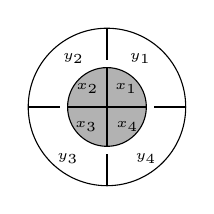
\begin{tikzpicture}
\draw(0,0) circle (1cm);
\draw[fill=black!30](0,0) circle (0.5cm);
\foreach \p in {0,90,180,270}
\draw[black](0,0)--(\p:0.5);
\foreach \p in {0,90,180,270}
\draw[black](\p:1)--(\p:0.6);
\coordinate[label=\tiny{$x_1$}](x1) at(10:0.25);
\coordinate[label=\tiny{$x_2$}](x2) at(170:0.25);
\coordinate[label=left:\tiny{$x_3$}](x3) at(270:0.25);
\coordinate[label=right:\tiny{$x_4$}](x4) at(270:0.25);
\coordinate[label=\tiny{$y_1$}](y1) at(45:0.6);
\coordinate[label=\tiny{$y_2$}](y2) at(135:0.6);
\coordinate[label=left:\tiny{$y_3$}](y3) at(250:0.7);
\coordinate[label=right:\tiny{$y_4$}](y4) at(290:0.7);
\end{tikzpicture}
\end{center}
\twoch{$ T_1,T_2,T_3,T_4$中至少有一个为正数}{$ T_1,T_2,T_3,T_4$中至少有一个为负数}{$ T_1,T_2,T_3,T_4$中至多有一个为正数}{$ T_1,T_2,T_3,T_4$中至多有一个为负数}
\qs 动点$ P $从$ A $出发,按逆时针方向沿周长为$ l $的平面图形运动一周,$ A,P $两点间的距离$ y $与动点$ P $所走过的路程$ x $的关系如图所示,那么动点$ P $所走的图形可能是\xx\par 
\begin{tikzpicture}
\coordinate[label=below left:$O$] (O) at(0,0);
\draw[->,>=latex](-0.2,0)--(2,0)node[below](x){$x$};
\draw[->,>=latex](0,-0.2)--(0,2)node[left](y){$y$};
\draw[domain=0:1.5]plot(\x,{-2*(\x-0.75)^2+2*0.75^2});
\draw[dashed]($(0.75,2*0.75^2)$)--(0.75,0)node[below](l){$ \tfrac{l}{2} $};
\end{tikzpicture}
\begin{tikzpicture}
\coordinate[label=left:$A$] (A)at (0,0);
\coordinate (B)at (2,0);
\coordinate (C)at (1,1.732);
\draw(A)--(B)--(C)--cycle;
\coordinate[label=right:$P$](P) at($(B)!0.3!(C)$);
\draw(A)--(P);
\coordinate[label=$(A)$](a) at(1,-0.8);
\begin{scope}[xshift=3 cm]
\coordinate[label=left:$A$] (A)at (0,0);

\draw(A)--++(1.732,0)--++(0,1.732)--++(-1.732,0)--cycle;
\coordinate[label=right:$P$](P) at(1.732,0.5);
\draw(A)--(P);
\coordinate[label=$(B)$](a) at(0.86,-0.8);
\end{scope}
\begin{scope}[xshift=6cm]
\coordinate[label=left:$A$] (A)at ($(245:0.866)+(0.866,0.866)$);
\coordinate (c)at (0.866,0.866);
\draw (c) circle (0.866);
\coordinate[label=right:$P$](P) at($(345:0.866)+(0.866,0.866)$);
\draw(A)--(P);
\coordinate[label=$(C)$](a) at(0.866,-0.8);
\end{scope}
\begin{scope}[xshift=9cm]
\coordinate[label=above:$A$] (A)at (0.866,0);
\coordinate (B)at (0.866,0.866);
\draw (B) ellipse (1.2 and 0.866);
\coordinate[label=right:$P$](P) at(2.066,0.866);
\draw(A)--(P);
\coordinate[label=$(D)$](a) at(0.866,-0.8);
\end{scope}
\end{tikzpicture}
\qs 已知函数$f(x)=\Bigg\{\begin{aligned}
&\log_ax,&x>0,\\
&\abs{x+3},&-4\le x<0.
\end{aligned}(a>0\text{且}a\ne1)$.若函数$f(x)$的图象上有且仅有两个点关于$y$轴对称,则$ a $的取值范围是\xx
\onech{$ \left(0,1\right)$}{$ \left(1,4\right)$}{$ \left(0,1\right)\cup\left(1,+\infty\right)$}{$ \left(0,1\right)\cup\left(1,4\right)$}
\qs $ S(A) $表示集合$ A $中所有元素的和,且$ A\subseteq\left\{1,2,3,4,5\right\} $,若$ S(A)$能被$ 3 $整除,则符合条件的非空集合$ A $的个数是\xx
\onech{$ 10$}{$ 11$}{$ 12$}{$ 13$}
\qs 已知一位手机用户前四次输入四位数字手机密码均不正确,第五次输入密码正确,手机解锁.事后发现前四次输入的密码中,每次都有两个数字正确,但它们各自的位置均不正确.已知前四次输入的密码分别为$ 3406,1630,7364,6173, $则正确的密码中一定含有的数字为\xx
\onech{$ 4,6$}{$ 3,6$}{$ 3,7$}{$ 1,7$}
\qs 据统计某超市两种蔬菜$ A,B $连续$ n $天价格分别为$ a_1,a_2,a_3,\cdots,a_n $和$ b_1,b_2,b_3,\cdots,b_n $,令$ M=\left\{m\left|a_m<b_m,m=1,2,\cdots,n\right.\right\} $,若$ M $中元素个数大于$ \dfrac{3}{4}n $,则称蔬菜$ A $在这$ n $天的价格低于蔬菜$ B $的价格,记作$ A\prec B $,现有三种蔬菜$ A,B,C $,下列说法正确的是\xx
\fourch{若$A\prec B,B\prec C $,则$ A\prec C $}{若$A\prec B,B\prec C $同时不成立,则$ A\prec C$不成立}{$A\prec B,B\prec A $可同时不成立}{$A\prec B,B\prec A $可同时成立}
\qs 已知甲、乙两个容器,甲容器的容量为$ x $,装满纯酒精,乙容器容量为$ z $,其中装有体积为$ y $的水($x,y<z$,单位:$ L $).现将甲容器中的液体倒入乙容器中,直至甲容器中液体倒完或乙容器盛满,搅拌使乙容器中两种液体充分混合,再将乙容器中的液体倒入甲容器中直至倒满,搅拌使甲容器中液体充分混合,如此称为一次操作,假设操作过程中溶液体积变化忽略不计,设经过$ n\left(n\in\mathbf{N^+}\right) $次操作之后,乙容器中含有纯酒精$ a_n $(单位:$L$).下列关于数列$ \left\{a_n\right\} $的说法正确的是\xx
\fourch{当$ x=y=a $时,数列$\{a_n\}$有最大值$ \dfrac{a}{2} $}{设$ b_n=a_{n+1}-a_n\left(n\in\mathbf{N^+}\right) $,则数列$\{b_n\}$为递减数列}{对任意的$ n\in\mathbf{N^+} $,始终有$ a_n\le\dfrac{xy}{z} $}{对任意的$ n\in\mathbf{N^+} $,始终有$ a_n\le\dfrac{xy}{x+y} $}
\qs 中国古代儒学家要求学生掌握六种基本才艺,礼、乐、射、御、书、数,简称“六艺”.某中学为弘扬“六艺”的传统文化,分别进行了主题为"礼、乐、射、御、书、数”六场传统文化知识的比赛.现有甲、乙、丙三位选手进入了前三名的最后角逐,规定:每场知识竞赛前三名的得分都分别是$ a,b,c (a>b>c\text{且}a,b,c\in \mathbf{N^*})$;选手最后得分为各场得分之和.在六场比赛后,已知甲最后得分为$26$分,乙和丙最后得分都为$11$分,且乙在其中一场比赛中获得第一名,则下列说法中正确的是\xx
\fourch{每次比赛第一名得分$a$为$4$}{甲可能有一场比赛获得第二名}{乙有四场比赛获得第三名}{丙可能有一场比赛获得第一名}
\qs 有三只股票$ A,B,C ,\text{共}28$位股民的持有情况如下:每位股民至少持有其中一支股票,在不持有$ A $股票的人中,持有$ B $股票的人数是持有$ C $股票的人数的$ 2 $倍.在持有$ A $股票的人中,只持有$ A $股票的人数比除了持有$ A $股票外,同时还持有其它股票的人数多$ 1 $.在只持有一支股票的人中,有一半持有$ A $股票.~则只持有$ B $股票的股民人数是\xx
\onech{$ 7$}{$ 6$}{$ 5$}{$ 4$}
\qs 在四边形$ ABCD $中,$ AB=2 $.若$ \vv{DA}=\dfrac{1}{2}(\vv{CA}+\vv{CB}) $,则$ \vv{AB}\bm{\cdot}\vv{DC} =$\tk.
\qs 已知函数$f(x)$的定义域为$ \mathbf{R} $,当$ x<0 $时,$f(x)=\ln (-x)+x $;当$ -e\le x\le e $时,$ f(-x)=-f(x) $;当$ x>1 $时,$ f(x+2)=f(x) $,则$f(8)=$\tk.
\qs 已知$ O $为坐标原点,点$ P $为直线$ 2x+y-2=0 $上的任意一点,非零向量$ \bm{a}=(m,n) .$若$ \vv{OP}\bm{\cdot a} $恒为定值,则$ \dfrac{m}{n}= $\tk.
\qs 已知函数$f(x)=\ln x+2x-6$的零点在区间$ \left(\dfrac{k}{2},\dfrac{k+1}{2}\right)~\left(k\inZ\right) $内,那么$ k= $\tk.
\qs 已知$ O $为$\triangle ABC$的外心,且$ \vv{BO}=\lambda \vv{BA}+\mu \vv{BC} $.\\
\ding{192}~若$ \angle C=90^{\circ} $,则$ \lambda+\mu $=\tk;\\
\ding{193}~若$ \angle ABC =60^{\circ}$,则$ \lambda+\mu $的最大值是\tk.
\qs 已知椭圆$ G:\dfrac{x^2}{6}+\dfrac{y^2}{b^2}=1~\left(0<b<\sqrt{6}\right) $的两个焦点分别为$ F_1,~F_2 $,短轴的两个端点分别为$ B_1,~B_2 $,点$ P $在椭圆$ G $上,且满足$ \abs{PB_1}+\abs{PB_2} =\abs{PF_1}+\abs{PF_2}$.当$ b $变化时,给出下列三个命题:\\
\ding{192}~点$ P $的轨迹关于$y$轴对称;\\
\ding{193}~存在$ b $使得椭圆$ G $上满足条件的点$ P $仅有$ 2 $个;\\
\ding{194}~$ \abs{OP} $的最小值为$ 2 $.\\
其中,所有正确命题的序号是\tk.
\qs 已知函数$f(x)=\Bigg\{\begin{aligned}
&-(x-1)^2+2,&x\le1,\\
&\dfrac{1}{x}+1,&x>1.
\end{aligned}$下列四个命题:\\
\ding{192}~$ f\left(f(1)\right) >f(3)$;\\
\ding{193}~$ \exists x_0\in\left(1,+\infty\right),f'(x_0)=-\dfrac{1}{3} $;\\
\ding{194}~$ f(x)$的极大值点为$ x=1 $;\\
\ding{195}~$ \forall x_1,x_2\in\left(0,+\infty\right),\abs{f(x_1)-f(x_2)}\le1 $.\\
其中正确的有\tk.(写出所有正确命题的序号)
\qs 若$x,y$满足$\begin{dcases}
y\ge1,\\
y\le x-1,\\
x+y\le m.
\end{dcases}$且$ z=x^2+y^2 $的最大值为$ 	10,~ $则$ m= $\tk.
\qs 在平面直角坐标系$xOy$中,点$ M $不与点$ O $重合,称射线$ OM $与圆$ x^2+y^2=1 $的交点$ N $为点$ M $的“中心投影点”.
\begin{parts}
\part 点$ M(1,\sqrt{3}) $的“中心投影点”为\tk;
\part 曲线$ x^2-\dfrac{y^2}{3}=1 $上的“中心投影点”构成的曲线的长度是\tk.
\end{parts}
\qs 设$ P $为曲线$ C_1 $上的动点,$ Q $为曲线$ C_2 $上的动点,则称$ \abs{PQ} $的最小值为曲线$ C_1,C_2 $之间的距离,记作$ d(C_1,C_2) $.若$ C_1:x^2+y^2=2,C_2:(x-3)^2+(y-3)^2=2, $则$ d(C_1,C_2)= $\tk;若$ C_3:e^x-2y=0,C_4:\ln x+\ln 2=y,~ $则$ d(C_3,C_4)= $\tk.
\qs 已知函数$f(x)=\begin{dcases}
\abs{x-1},&x\in\left(0,2\right],\\
min\left\{\abs{x-1},\abs{x-3}\right\},&x\in\left(2,4\right],\\
min\left\{\abs{x-3},\abs{x-5}\right\},&x\in\left(4,+\infty\right).
\end{dcases}$\\
\ding{192}~若$f(x)=a$有且只有$ 1 $个实根,则实数$ a $的取值范围是\tk;\\
\ding{193}~若关于$ x $的方程$ f(x+T)=f(x) $有且只有$ 3 $个不同的实根,则实数$ T $的取值范围是\tk.
\qs 已知两个集合$ A,B $满足$ B\subseteq A $.若对任意的$ x\in A $,存在$ a_i,a_j\in B(i\ne j) ,$使得$ x=\lambda_1a_i+\lambda_2a_j(\lambda_1,\lambda_2\in\left\{-1,0,1\right\}) $,则称$ B $为$ A $的一个基集.若$ A=\left\{1,2,3,4,5,6,7,8,9,10\right\} $,则其基集$ B $的元素个数的最小值是\tk.
\qs 如图,在棱长为$ 1 $的正方体$ABCD-A_1B_1C_1D_1$中,点$ P $是线段$ BD_1 $上的动点,当$ \triangle PAC $在平面$ DC_1,~BC_1,~AC $上的正投影都为三角形时,将它们的面积分别记为$ S_1,~S_2,~S_3 $.
\begin{parts}
\part 当$ BP =\dfrac{\sqrt{3}}{3}$时,$ S_1 $\tk$ S_2 $~(填“>”或“=”或“<”);
\part $ S_1+S_2+S_3 $的最大值是\tk.
\end{parts}
\begin{center}
\begin{tikzpicture}
\tikzmath{
\a=cos(45);
\b =sin(45);
\c=1*\a ;
\d =1*\b ;
}
\coordinate[label=left:$A$](A) at (0,0);
\coordinate[label=right:$B$](B) at (2,0);
\coordinate[label=above right:$D$](D) at(\c,\d);
\coordinate[label={right,above}:$C$](C) at($(B)+(\c,\d)$);
\foreach \p in{B,C}
\coordinate[label=right:$\p_1$](\p_1) at($(\p)+(0,2)$);
\foreach \p in{A,D}
\coordinate[label=left:$\p_1$](\p_1) at($(\p)+(0,2)$);
\draw (A)--(B)--(C)--(D)--cycle;
\draw (A_1)--(B_1)--(C_1)--(D_1)--cycle;
\foreach \p in{A,B,C,D}
\draw (\p)--(\p_1);
\draw[dashed] (B)--(D_1);
\coordinate[label=above:$P$](P) at($(B)!0.2!(D_1)$);
\draw[fill] (P) circle (1pt);
\draw[dashed](A)--(C);

\end{tikzpicture}
\end{center}
\qs 如图,在棱长为$ 1 $的正方体$ABCD-A_1B_1C_1D_1$中,$ E $是对角线$ B_1D $上的一点,$ M,N $为对角线$ AC $上的两个动点,且线段$ MN $的长度为$ 1 .$
\begin{parts}
\part 当$ N $为对角线$ AC $的中点且$ DE=\sqrt{2} $时,则三棱锥$ E-DMN $的体积是\tk;
\part 当三棱锥$ E-DMN $的体积为$ \dfrac{1}{3} $时,则$ DE= $\tk.
\end{parts}
\begin{center}
\begin{tikzpicture}
\tikzmath{
\a=cos(45);
\b =sin(45);
\c=1*\a ;
\d =1*\b ;
}
\coordinate[label=left:$A$](A) at (0,0);
\coordinate[label=right:$D$](D) at (2,0);
\coordinate[label=above right:$B$](B) at(\c,\d);
\coordinate[label={right,above}:$C$](C) at($(D)+(\c,\d)$);
\foreach \p in{D,C}
\coordinate[label=right:$\p_1$](\p_1) at($(\p)+(0,2)$);
\foreach \p in{A,B}
\coordinate[label=left:$\p_1$](\p_1) at($(\p)+(0,2)$);
\draw (A)--(B)--(C)--(D)--cycle;
\draw (A_1)--(B_1)--(C_1)--(D_1)--cycle;
\foreach \p in{A,B,C,D}
\draw (\p)--(\p_1);
\draw[dashed] (B_1)--(D);
\coordinate[label=above:$E$](E) at($(B_1)!0.7!(D)$);
\coordinate[label=below:\small$N$](N) at($(A)!0.45!(C)$);
\coordinate[label=above:\small$M$](M) at($(A)!0.3!(C)$);
\draw[densely dashed](E)--(M) (E)--(N) (D)--(M) (D)--(N);
%\draw[fill] (P) circle (1pt);
\draw[dashed](A)--(C);

\end{tikzpicture}
\end{center}



\newpage
\section{解答题}
%\begin{questions}
\qs 已知动点$ M $到点$ N(1,0) $和直线$ l:x=-1 $的距离相等.
\begin{parts}
\part 求动点$ M $的轨迹$ E $的方程;
\part 已知不与$ l $垂直的直线$ l' $与曲线$ E $有唯一公共点$ A $,且与直线$ l $的交点为$ P $,以线段$ AP $为直径的作圆$ C .$判断点$ N $和圆$ C $的位置关系,并证明你的结论.
\end{parts}
\kongbai
\qs 已知$ F_1(-1,0) ,F_2(1,0)$分别是椭圆$ C:\dfrac{x^2}{a^2}+\dfrac{y^2}{3}=1~(a>0) $的左、右焦点.
\begin{parts}
\part 求椭圆$ C $的方程;
\part 若$ A,B $分别在直线$ x=-2 $和$ x=2 $上,且$ AF_1\bot BF_1 $.\begin{enumerate}[(i)]
\item 当$ \triangle ABF_1 $为等腰三角形时,求$ \triangle ABF_1 $的面积;
\item 求点$ F_1,F_2 $到直线$ AB $距离之和的最小值.
\end{enumerate}
\end{parts}
\kongbai
\qs 已知椭圆$C$:$\dfrac{x^2}{a^2}+\dfrac{y^2}{b^2}=1~(a>b>0)$的短轴长为$ 2\sqrt{3} $,右焦点为$ F(1,0) $,点$ M $是椭圆$ C $上异于左、右顶点$ A,B $的一点.
\begin{parts}
\part 求椭圆$C$的方程;
\part 若直线$ AM $与直线$ x=2 $交于点$ N $,线段$ BN $的中点为$ E $.证明:点$ B $关于直线$ EF $的对称点在直线$ MF $上.
\end{parts}
\kongbai 
\qs 已知椭圆$ E:mx^2+y^2=1(m>0) $.
\begin{parts}
\part 若椭圆$ E $的右焦点坐标为$ \left(\sqrt{3},0\right), ~$求$ m $的值;
\part 由椭圆$ E $上不同三点构成的三角形称为椭圆的内接三角形.若以$ B(0,1) $为直角顶点的椭圆$ E $的内接等腰直角三角形恰有三个,求$ m $的取值范围.
\end{parts}
\kongbai
\qs 已知椭圆$ E $的右焦点与抛物线$ y^2=4x $的焦点重合,点$ M(1,\dfrac{3}{2}) $在椭圆$ E $上.
\begin{parts}
\part 求椭圆$ E $的方程;
\part 设$ P(-4,0) $,直线$ y=kx+1 $与椭圆$ E $交于$ A,B $两点,若直线$ PA,~PB $均与圆$ x^2+y^2=r^2~(r>0) $相切,求$ k $的值.
\end{parts}
\kongbai
\qs 已知椭圆$ C:\dfrac{x^2}{4}+\dfrac{y^2}{3}=1 $,点$ P(4,0) $,过右焦点$ F $作与$y$轴不垂直的直线$ l $交椭圆$ C $于$ A,B $两点.
\begin{parts}
\part 求椭圆$C$的方程;
\part 求证:以坐标原点$ O $为圆心与直线$ PA $相切的圆,必与直线$ PB $相切.
\end{parts}
\kongbai
\qs 已知椭圆$W$:$\dfrac{x^2}{a^2}+\dfrac{y^2}{b^2}=1~(a>b>0)$的上下顶点分别为$ A,B $,且点$ B(0,-1) .F_1,F_2$分别为椭圆$W$的左、右焦点,且$ \angle F_1BF_2 =120^{\circ}$.
\begin{parts}
\part 求椭圆$W$的方程;
\part 点$ M $是椭圆上异于$ A,B $的任意一点,过点$ M $作$ MN \bot y$轴于$ N,~E $为线段$ MN $的中点.直线$ AE $与直线$ y=-1 $交于点$ C,~G $为线段$ BC $的中点,$ O $为坐标原点,求$ \angle OEG $的大小.
\end{parts}
\kongbai
\qs 已知椭圆$ W:\dfrac{x^2}{4}+\dfrac{y^2}{b^2}=1 $的一个焦点坐标为$ (\sqrt{3},0) .$
\begin{parts}
\part 求椭圆$ W $的方程和离心率;
\part 若椭圆$ W $与$y$轴交于$ A,B $两点($A$点在$ B $点上方),$ M $是椭圆上异于$ A,B $的任意一点,过点$ M $作$ MN\bot y $轴于点$ N, ~E $为线段$ MN $的中点.直线$ AE $与直线$ y=-1 $交于点$ C,~G $为线段$ BC $的中点,$ O $为坐标原点,求$ \angle OEG $的大小.
\end{parts}
\kongbai
\qs 在平面直角坐标系$xOy$中,抛物线$ C $的顶点是原点,以$x$轴为对称轴,且经过点$ P\left(1,2\right) .$
\begin{parts}
\part 求抛物线$ C $的方程;
\part 设点$ A,B $在抛物线$ C $上,直线$ PA,~PB $分别与$y$轴交于点$ M,N,~ \abs{PM}=\abs{PN}$.求直线$ AB $的斜率.
\end{parts}
\kongbai
\qs 已知函数$f(x)=\dfrac{1}{3}x^3+\dfrac{1}{2}x^2-2x+1$.
\begin{parts}
\part 求函数$f(x)$的单调区间;
\part 当$ 0<a<\dfrac{5}{2} $时,求函数$f(x)$在区间$ \left[-a,a\right] $上的最大值.
\end{parts}
\kongbai
\qs 已知函数$f(x)=e^{ax}-x$.
\begin{parts}
\part 若曲线$y=f(x)$在$ (0,f(0)) $处的切线$ l $与直线$ x+2y+3=0 $垂直,求$ a $的值;
\part 当$ a\ne 1 $时,求证:存在实数$ x_0 $使$f(x_0)<1$.
\end{parts}
\kongbai
\qs 设函数$f(x)=(x^2+ax-a)e^{-x}(a\inR)$.
\begin{parts}
\part 当$ a=0 $时,求曲线$y=f(x)$在点$ \left(-1,f(-1)\right) $处的切线方程;
\part 设$g(x)=x^2-x-1$,若对任意的$ t\in\left[0,2\right] $,存在$ s\in\left[0,2\right] $使得$ f(s)\ge g(t) $成立,求$ a $的取值范围.
\end{parts}
\kongbai
\qs 设函数$f(x)=(x-a)e^x,a\inR$.
\begin{parts}
\part 当$ a=1 $时,试求$f(x)$的单调区间;
\part 试求$f(x)$在$ \left[1,2\right] $上的最大值;
\part 当$ a=1 $时,求证:对于$ \forall x\in \left[-5,+\infty\right),~f(x)+x+5\ge -\dfrac{6}{e^5} $恒成立.
\end{parts}
\kongbai 
\qs 已知函数$f(x)=e^x-a\ln x-a$.
\begin{parts}
\part 当$ a=e $时,求曲线$y=f(x)$在点$ \left(1,f(1)\right) $处的切线方程;
\part 证明:对于$ \forall a\in\left(0,e\right) ,~f(x)$在区间$ \left(\dfrac{a}{e},1\right) $上有极小值,且极小值大于$ 0 $.
\end{parts}
\kongbai
\qs 已知函数$f(x)=\dfrac{\ln x }{ax}(a>0)$.
\begin{parts}
\part 当$ a=1 $时,求曲线$y=f(x)$在点$ \left(1,f(1)\right) $处的切线方程;
\part 若$f(x)<\dfrac{1}{\sqrt{x}}$恒成立,求$ a $的取值范围;
\part 证明:总存在$ x_0 $,使得当$ x\in\left(x_0,+\infty\right) $,恒有$ f(x)<1. $
\end{parts}
\kongbai
\qs 已知函数$f(x)=e^x+x^2-x,~g(x)=x^2+ax+b(a\inR,b\inR)$.
\begin{parts}
\part 当$ a=1 $时,求函数$F(x)=f(x)-g(x)$的单调区间;
\part 若曲线$y=f(x)$在点$ (0,1) $处的切线$ l $与曲线$y=g(x)$切于点$ (1,c) $,求$ a,b,c $的值;
\part 若$f(x)>g(x)$恒成立,求$ a+b $的最大值.
\end{parts}
\kongbai
\qs 已知函数$f(x)=x\ln x,~g(x)=\dfrac{a}{2}x^2+x-a~(a\inR)$.
\begin{parts}
\part 若直线$x=m~(m>0)$与曲线$y=f(x)$和$y=g(x)$分别交于$ M,N $两点.设曲线$y=f(x)$在点$ M $处的切线为$ l_1 $,$y=g(x)$在点$ N $处的切线为$ l_2 $.
\begin{enumerate}[(i)]
\item 当$ m=e $时,若$ l_1\bot l_2 $,求$ a $的值;
\item 若$ l_1\sslash l_2 $,求$ a $的最大值;
\end{enumerate}
\part 设函数$h(x)=f(x)-g(x)$在其定义域内恰有两个不同的极值点$ x_1,x_2 $,且$ x_1<x_2 $.若$ \lambda>0, $且$ \lambda \ln x_2-\lambda>1-\ln x_1 $恒成立,求$ \lambda $的取值范围.
\end{parts}
\kongbai 
\qs 已知函数$f(x)=\left(x^2+ax-a\right)\bm{\cdot}e^{1-x},~\text{其中}a\inR$.
\begin{parts}
\part 求函数$f'(x)$的零点个数;
\part 证明:$ a\ge0 $是函数$f(x)$存在最小值的充分而不必要条件. 
\end{parts}
\end{questions}
\end{document}